\section{Vector Fields} \label{S:12.1.VectorFields}


\vspace*{-14 pt}
\framebox{\hspace*{3 pt}
\parbox{6.25 in}{\begin{goals}
\item What is a vector field?
\item How do we draw a vector field?
\item What are some familiar contexts in which vector fields arise?
\end{goals}} \hspace*{3 pt}}

\subsection*{Introduction}

Thus far vectors have played a central role in our study of
multivariable calculus. We know how to do operations on vectors
(addition, scalar multiplication, dot product, etc.), and we have seen
how vectors can be used to describe curves in $\R^2$ and $\R^3$. The
examples of using vectors to describe curves was our first example of
a vector-valued function. That is, a curve $\vr(t)$ is really a
function that takes as input a real number and produces a vector in
$\R^2$ or $\R^3$. In this section we will expand our understanding of
vector-valued functions to take as input a point $(x,y)$ in $\R^2$ or
a point $(x,y,z)$ in $\R^3$ and produce a vector (typically in $\R^2$
or $\R^3$, respectively).


\begin{pa} \label{PA:12.1}
It's common for weather forecasters to discuss the wind \emph{speed}, but as any student who has gotten this far in the text will know, this nomenclature is imprecise. It's not terribly helpful to tell someone the wind is blowing at $10$ km/h without telling them the direction in which the wind is blowing. If you're trying to make a decision based on what the wind is doing, you need to know about the direction as well. (Perhaps you are taking off in a hot air balloon and need to know which direction the chase team should head to keep track of you.) Because of the swirling nature of wind, it makes sense to give the wind \emph{velocity} at every point in a region (two-dimensional or three-dimensional). 

\ba
\item \label{enum:PA12.1F} Suppose that given a point $(x,y)$ in the plane, you know that the wind velocity at that point is given by the vector $\vF(x,y) = \langle y,x\rangle$. For example, we'd then know that at the point $(1,-1)$, the wind velocity is $\vF(1,-1) = \langle -1,1\rangle$. In the table below, fill in the wind velocity vectors for the given points.
  \begin{center}
    \begin{tabular}{c|c|c|c|c|c}
      $(x,y)$ & $(2,1)$ & $(0,0)$ & $(-1,2)$ & $(3,-1)$ & $(-2,-1)$\\\hline
$\vF(x,y)$ & & & & &
    \end{tabular}
  \end{center}
\item \label{enum:PA12.1G} Suppose that we associate the vector $\vG(x,y) = -x\vj$ to a point $(x,y)$ in the plane. Complete the table below by giving the vector associated to each of the given points.
  \begin{center}
    \begin{tabular}{c|c|c|c|c|c|c|c|c}
      $(x,y)$ & $(-2,0)$ & $(-1,2)$ & $(0,-2)$ & $(1,1)$ & $(2,3)$ & $(3,2)$ & $(-1,0)$ & $(1,3)$\\\hline
$\vG(x,y)$ & & & & & & &
    \end{tabular}
  \end{center}

\saveCount
\ea

A table of values of these vector-valued functions is useful, but perhaps even better is a method of visualizing the vectors. In keeping with our wind velocity analogy, if $\vF(2,1) = \langle 1,2\rangle$, we draw the vector $\langle 1,2\rangle$ with its tail at the point $(2,1)$. 

\ba
\restoreCount
\item Using the first set of axes in Figure~\ref{fig:PA12.1a}, plot the vectors $\vF(x,y)$ for the five points in the table in part \ref{enum:PA12.1F}. The example $\vF(1,-1) = \langle -1,1\rangle$ is drawn for you.
\item Using the second set of axes in Figure~\ref{fig:PA12.1a}, plot the vectors $\vG(x,y)$ for the eight points in the table in part \ref{enum:PA12.1G}. 
% TODO: Actually include the promised vector on the left grid.
  \begin{figure}[h]
    \centering
    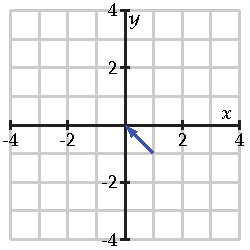
\includegraphics{figures/PA12-1F-axes.pdf}\hspace{0.5in}    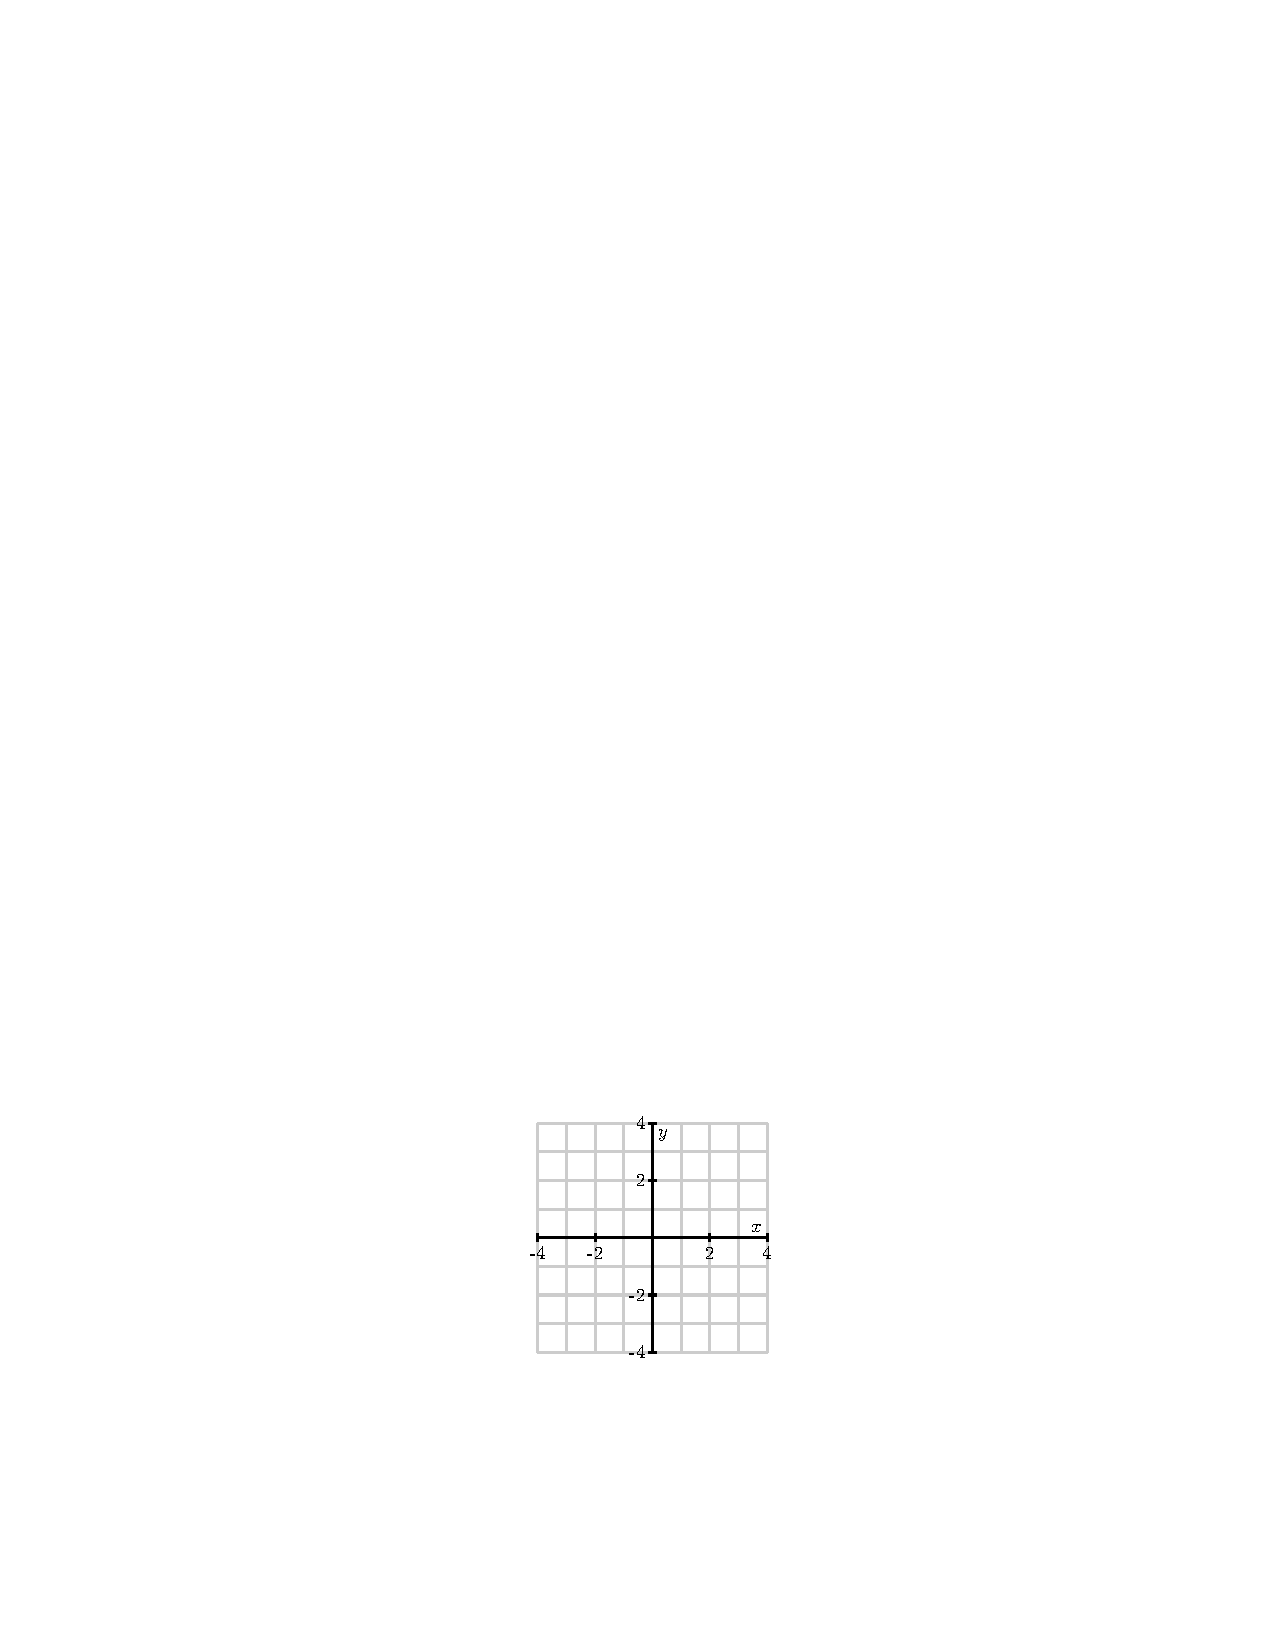
\includegraphics{figures/PA12-1G-axes.pdf}
    \caption{Axes for plotting some vectors from $\vF(x,y)$ and $\vG(x,y)$.}
    \label{fig:PA12.1a}
  \end{figure}
\ea
\end{pa} 
\afterpa 
%%% Local Variables:
%%% mode: latex
%%% TeX-master: "../0_AC_MV"
%%% End:


\subsection*{Examples of Vector Fields}

As Preview Activity~\ref{PA:12.1} showed you, one example of a time
where it makes sense to associate a vector to each point in a region
is a \emph{velocity vector field} $\vF(x,y)$ or $\vF(x,y,z)$, where
the vector associated to the point $(x,y)$ or $(x,y,z)$ is the
velocity of something at that point. Wind velocity is one example, but
another example would be the velocity of a flowing fluid.
Figure~\ref{fig:12.1.fluid-velocity} shows such a velocity vector
field. Technically, it only shows some of the vectors in the vector
field, since the figure would be unintelligible if all of the vectors
were shown. This is illustrated by the inset in the upper left corner,
which gives a better picture of what we would see if we zoomed in on
the red square of the main figure.

\begin{figure}[h]
  \centering
  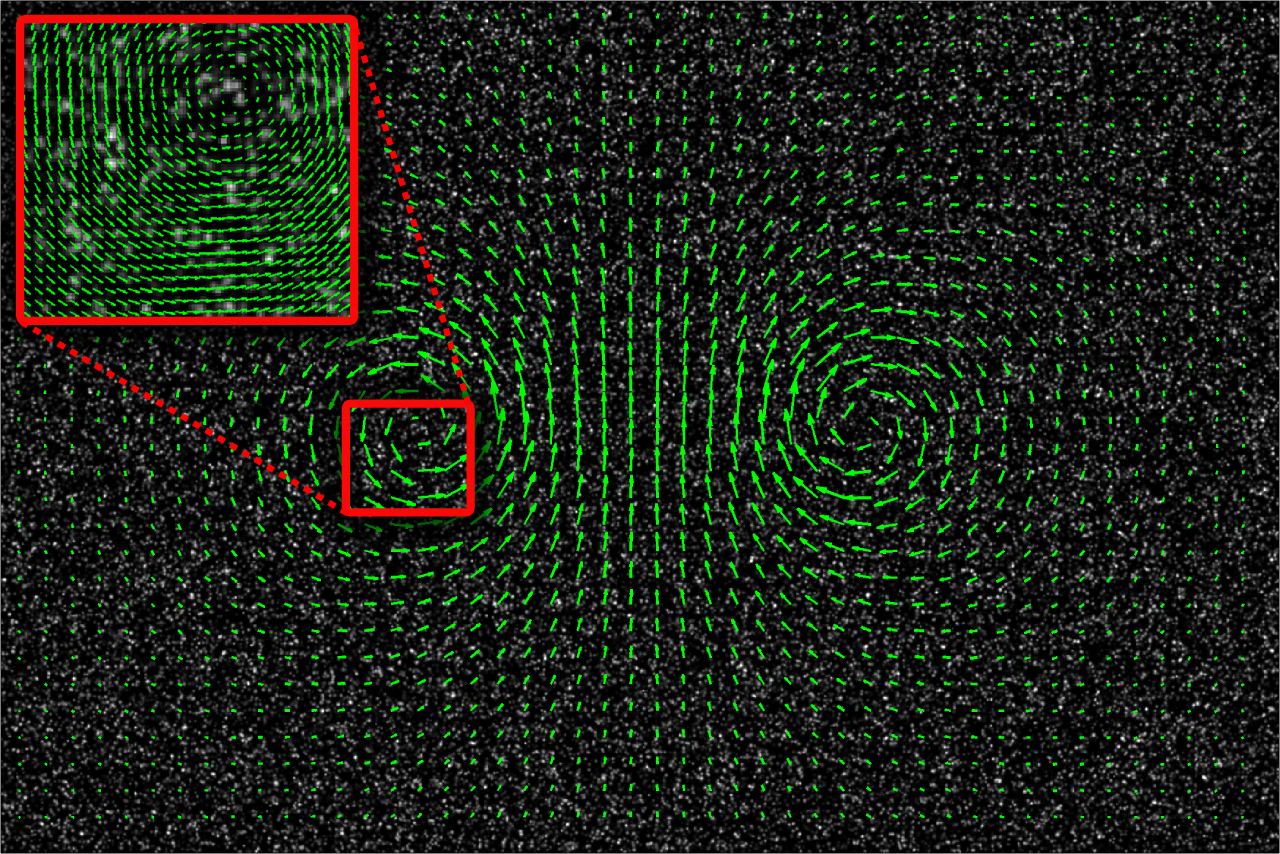
\includegraphics[width=0.9\linewidth]{figures/12_1_PIVlab_multipass.jpg}

  \vspace{-5pt}{\scriptsize \href{https://commons.wikimedia.org/wiki/File:PIVlab_multipass.jpg\#/media/File:PIVlab_multipass.jpg}{"PIVlab multipass" by Willa} - Own work. Licensed under CC-BY-SA 3.0 via Wikimedia Commons}
  \caption{An illustration of some of the vectors in a fluid velocity
    vector field.}
  \label{fig:12.1.fluid-velocity}
\end{figure}

Force fields, such as those created by gravity, are also examples of
vector fields. For example, the earth exerts a gravitational force on
objects. The force is directed from the center of the object to the
center of the earth, and its magnitude is determined by the distance
between the object and the earth. An illustration of this vector field
can be seen in Figure~\ref{fig:12.1.gravity}, where the earth is
positioned at the origin, but not shown. Notice that the vectors get
shorter as the distance from the origin increases, reflecting the fact
that the gravitational force is weaker at that distance.

\begin{figure}[h]
  \centering
  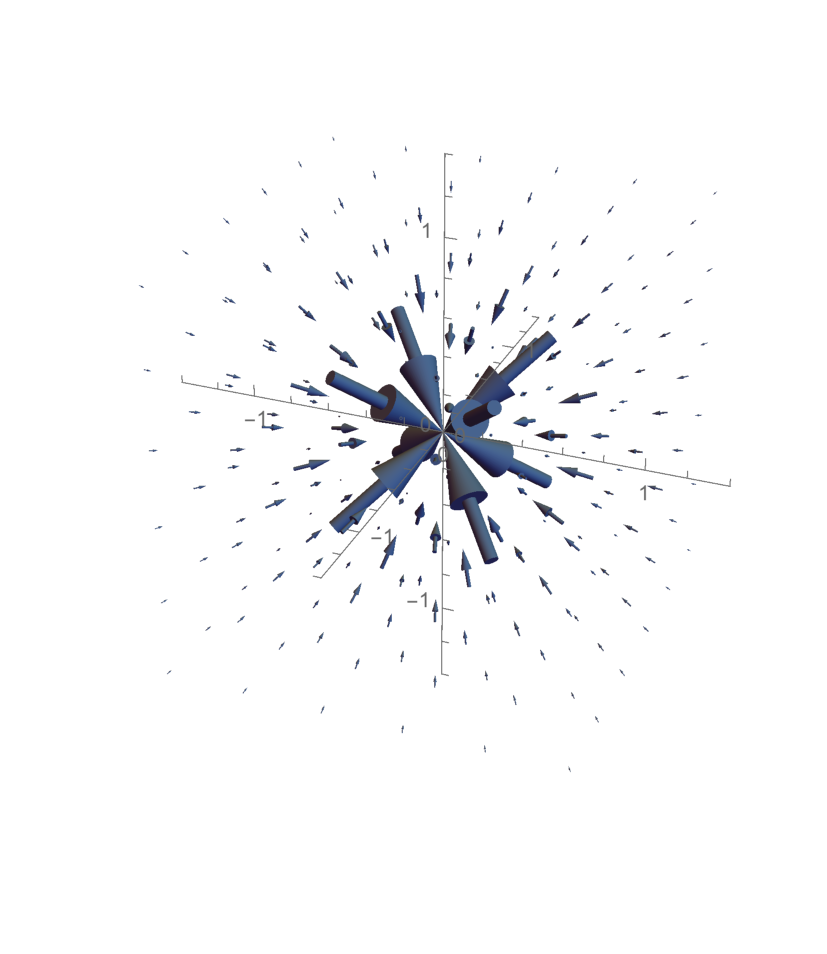
\includegraphics[width=0.4\linewidth]{figures/12_1_gravity_field.pdf}
  \caption{Gravitational vector field.}
  \label{fig:12.1.gravity}
\end{figure}

\subsection*{Mathematical Vector Fields}

As suggested in the introduction and Preview Activity~\ref{PA:12.1},
vector fields can be given by formulas.

\vspace*{5pt}
\nin \framebox{\hspace*{3 pt}
  \parbox{6.25 in}{\begin{definition} A
      \textbf{vector field}\index{vectorfield!definition} in $2$-space
      function whose value at a point $(x,y)$ is a $2$-dimensional
      vector $\vF(x,y)$. In $3$-space, a vector field is similarly a
      function $\vF(x,y,z)$ whose value at the point $(x,y,z)$ is a
      $3$-dimensional vector.
\end{definition} } \hspace*{3 pt}} \vspace*{5pt}

Since $\vF(x,y,z)$ is a vector, it has $\vi$, $\vj$, and $\vk$
components. Each of these components is a scalar function of the point
$(x,y,z)$, and so we will often write
\[\vF(x,y,z) = F_1(x,y,z)\vi + F_2(x,y,z)\vj + F_3(x,y,z)\vk.\]
For example, if $\vF(x,y,z) = \langle x^2,xy\sin(z),y^3\rangle$, then
$F_1(x,y,z) = x^2$, $F_2(x,y,z) = xy\sin(z)$, and $F_3(x,y,z) =
y^3$. Any time we are considering a vector field $\vF(x,y,z)$, the
definitions of functions $F_1$, $F_2$, and $F_3$ should be assumed in
this manner. (For a vector field $\vF(x,y)$ in $2$-space, we only have
the functions $F_1$ and $F_2$, defined analogously.)

\subsection*{Plotting Vector Fields}

Preview Activity~\ref{PA:12.1} gave you a chance to plot some vectors
in the vector fields $\vF(x,y) = \langle y,x\rangle$ and $\vG(x,y) =
\langle 0,-x\rangle$. It would be impossible to sketch \emph{all} of
the vectors in these vector fields, since there is one for every point
in the plane. In fact, even sketching by hand many more of the vectors
than you were asked to in the preview activity rapidly becomes
tedious. Fortunately, computer algebra systems can do a great job of
making such sketches. One thing to keep in mind, however, is that the
magnitudes of the vectors are typically scaled in these plots,
including plots of vector fields we will encounter later in the
text. To illustrate this, consider the two plots of the vector field
$\vF(x,y) = y\vi + x\vj$ in Figure~\ref{fig:12.1.scale-field}. 
\begin{figure}[h]
  \centering
  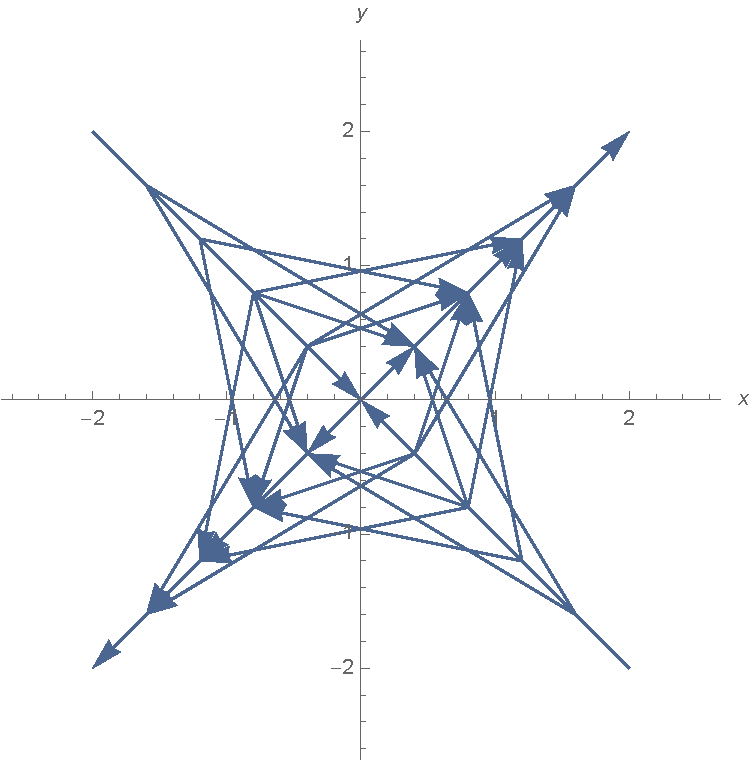
\includegraphics[width=0.3\linewidth]{figures/12_1_vecfield_unscaled.pdf}\hspace{0.2\linewidth}  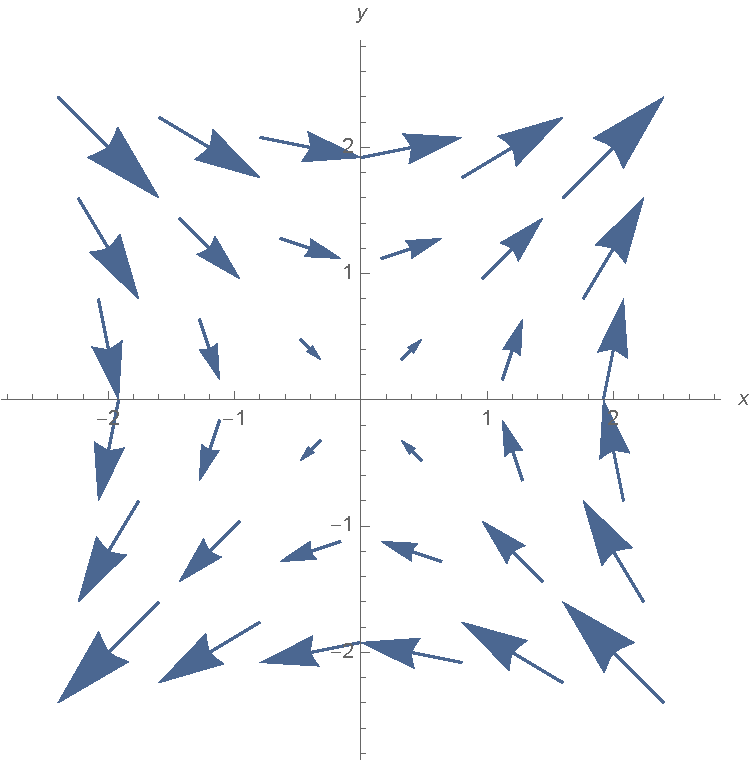
\includegraphics[width=0.3\linewidth]{figures/12_1_vecfield_scaled.pdf}
  \caption{Two plots of $\vF(x,y) = y\vi + x\vj$ from a computer
    algebra system}
  \label{fig:12.1.scale-field}
\end{figure}
The left plot shows some of the vectors but accurately depicts all of
their magnitudes, making the figure very hard to understand,
especially along the lines $y=x$ and $y=-x$. The plot on the right,
however, uses a uniform scaling to make the figure easier to read. As
before, each vector's direction is completely accurate, but now the
magnitudes are much smaller. However, the \emph{relative} magnitudes
are preserved, helping us to see that vectors farther from the origin
have larger magnitude than those closer to the origin.


\begin{activity} \label{A:12.1.1}  
\nin The plot in Figure~\ref{fig:12.1.circle} illustrates the vector
field $\vF(x,y) = y\vi -x\vj$.
\begin{figure}[h]
  \centering
  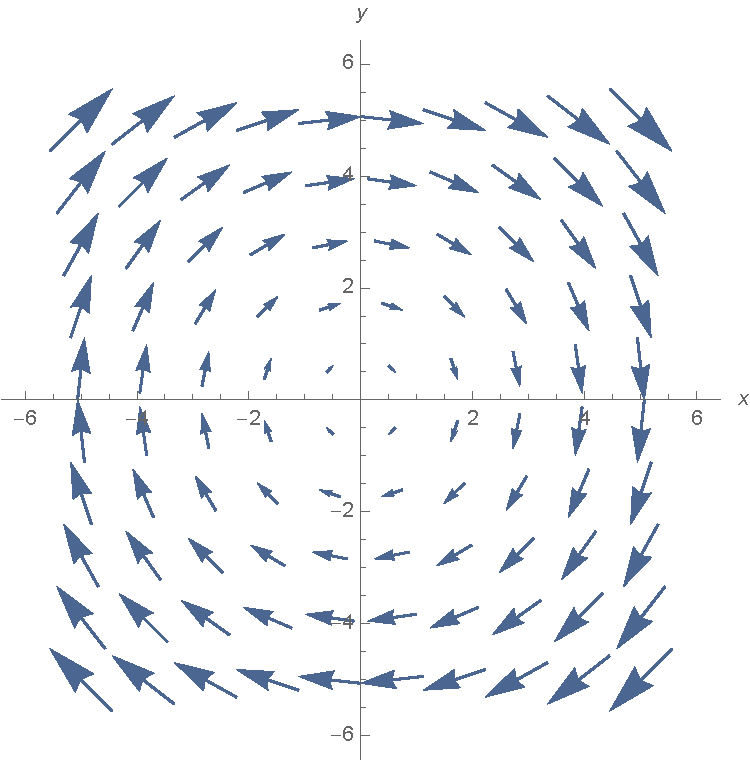
\includegraphics[width=0.35\linewidth]{12_1_circle.pdf}
  \caption{The vector field $y\vi-x\vj$}
  \label{fig:12.1.circle}
\end{figure}
\ba
\item Starting with one of the vectors near the point $(2,0)$, sketch
  a curve that follows the direction of the vector field $\vF$. To
  help visualize what you are doing, it may be useful to think of the
  vector field as the velocity vector field for some flowing water and
  that you are imagining tracing the path that a tiny particle
  inserted into the water would follow as the water moved it around.
\item Repeat the previous step for at least two other starting points
  not on the curve you previously sketched.
\item What shape do the curves you sketched in the previous two steps
  form?
\item Verify that $\vF(x,y)$ is orthogonal to $\langle x,y\rangle$.
\item What is the relationship between the function $f(x,y) = x^2 +
  y^2$ and the vector $x\vi + y\vj$? %(You might find it useful to
%  think about the vector $2x\vi + 2y\vj$ first.) 
\item What does this tell you about the relationship between
  $\vF(x,y)$ and circles centered at the origin?  What is the
  relationship between $|\vF(x,y)|$ and the radius of the appropriate circle?
\ea
\end{activity}
\begin{smallhint}

\end{smallhint}
\begin{bighint}

\end{bighint}
\begin{activitySolution}

\end{activitySolution}
\aftera
%%% Local Variables:
%%% mode: latex
%%% TeX-master: "../0_AC_MV"
%%% End:


\subsection*{Gradient Vector Fields}

Without using the terminology, we've actually already encountered one
very important family of vector fields a number of times. Given a function $f$ of two or three variables, the gradient of
$f$ is a vector field, since for any point where $f$ has first-order
partial derivatives, $\nabla f$ assigns a vector to that point.

\begin{activity} \label{A:12.1.2}  
\ba
\item In Figure~\ref{fig:12.1.level-curves} there are three sets of axes showing level
  curves for functions $f$, $g$, and $h$, respectively. Sketch at least six vectors
  in the gradient vector field for each function. In making your
  sketches, you don't have to worry about getting vector magnitudes
  precise, but you should ensure that the relative magnitudes (and directions) are
  correct for each function independently.
  \begin{figure}[h]
    \centering
    \parbox[t]{0.3\linewidth}{\centering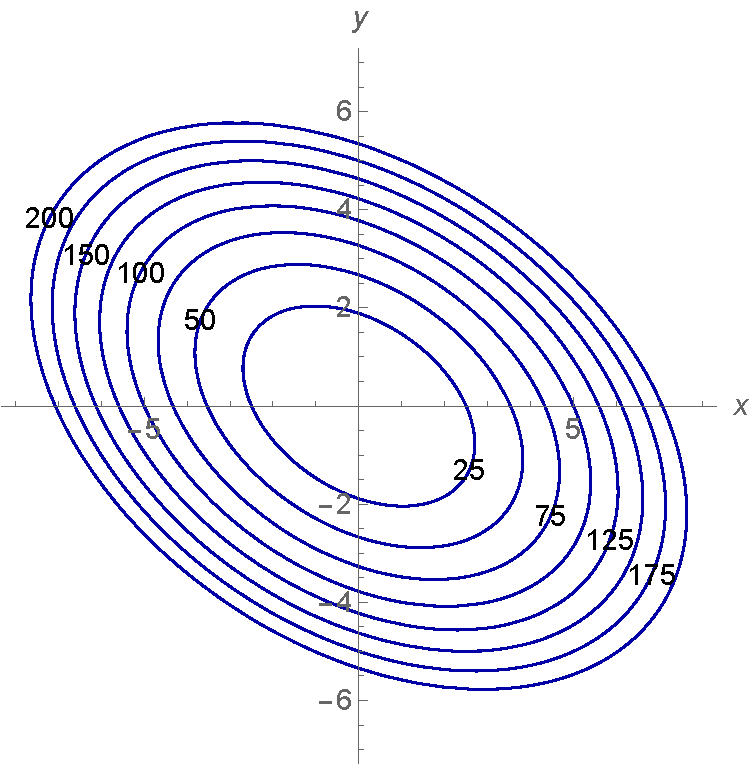
\includegraphics[width=\linewidth]{../figures/12_1_ellipses.pdf}\\\hspace{-4pt}$f$}\hspace{0.04\linewidth}\parbox[t]{0.3\linewidth}{\centering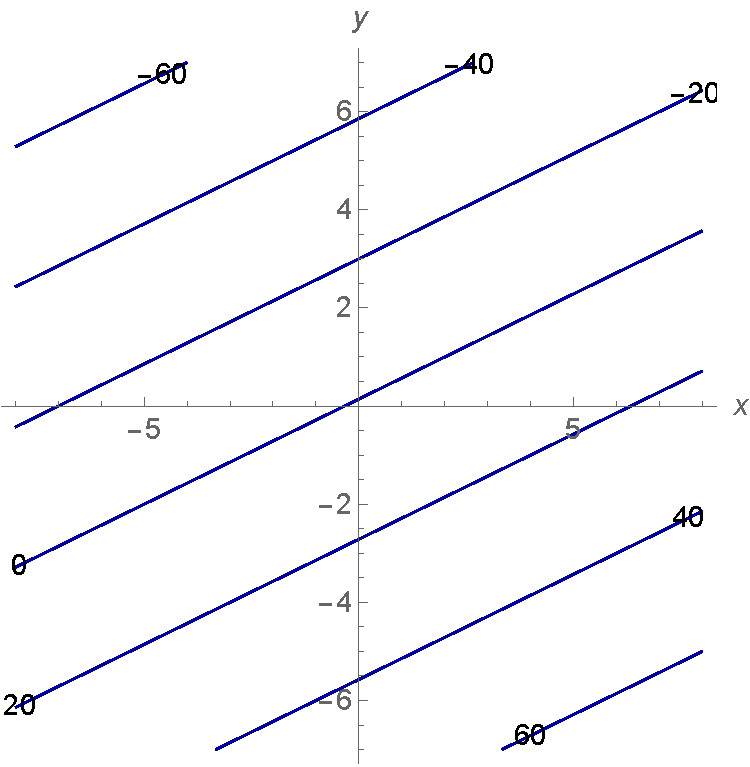
\includegraphics[width=\linewidth]{../figures/12_1_linear.pdf}\\\hspace{-4pt}$g$}\hspace{0.04\linewidth}\parbox[t]{0.3\linewidth}{\centering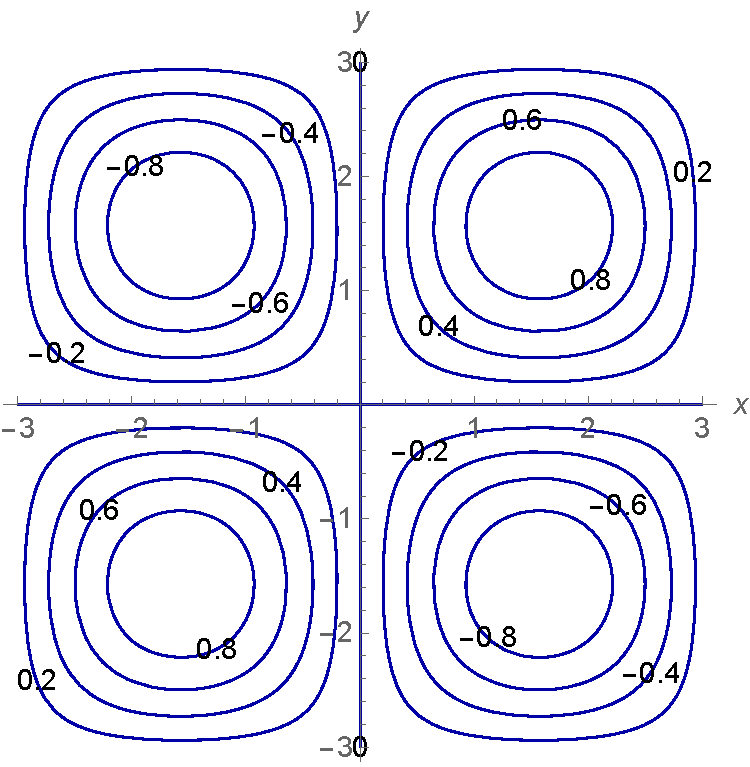
\includegraphics[width=\linewidth]{../figures/12_1_sine.pdf}\\\hspace{-3pt}$h$}
    \caption{Three sets of level curves}
    \label{fig:12.1.level-curves}
  \end{figure}
\item Verify that $\vF(x,y) = \langle 6xy,3x^2+9\sqrt{y}\rangle$ is a
  gradient vector field by finding a function $f$ such that $\nabla
  f(x,y) = \vF(x,y)$. For reasons originating in physics, such a
  function $f$ is called a \emph{potential function} for the vector
  field $\vF$.\label{part:A12.2-pot}
\item Is the function $f$ found in part \ref{part:A12.2-pot} unique?
  That is, can you find another function $g$ such that $\nabla g(x,y)
  = \vF(x,y)$ but $f\neq g$?
\item Is the vector field $\vF(x,y) = 6xy\vi +(2x+9\sqrt{y})\vj$ a
  gradient vector field? Why or why not?
\ea
\end{activity}
\begin{smallhint}

\end{smallhint}
\begin{bighint}

\end{bighint}
\begin{activitySolution}

\end{activitySolution}
\aftera
%%% Local Variables:
%%% mode: latex
%%% TeX-master: "../0_AC_MV"
%%% End:



%\nin \framebox{\hspace*{3 pt}
%\parbox{6.25 in}{
\begin{summary}
\item A $2$-dimensional vector field is a function defined on part of
  $\R^2$ whose value is a $2$-dimensional vector. A $3$-dimensional
  vector field is a function defined on part of $\R^3$ whose value is
  a $3$-dimensional vector.
\item Vector fields arise in familiar contexts such as wind velocity,
  fluid velocity, and gravitational force.
\item Vector fields are generally plotted in ways that ensure the
  direction and relative magnitudes of the vectors sketched are
  correct instead of ensuring that each vector's magnitude is
  depicted correctly.
\item The gradient of a function $f$ of two or three variables is a vector
  field defined wherever $f$ has partial derivatives.
\end{summary}
%} \hspace*{3 pt}}

\nin \hrulefill

%\input{exercises/9.2.Vectors(Ex)}

\clearpage

%%% Local Variables:
%%% mode: latex
%%% TeX-master: "0_AC_MV"
%%% End:
